% !TEX root = recipeUnderstanding.tex


\section{Experiments}
In order to experiment the proposed method, we first collected a dataset (details in Section~\ref{dataset:sec}). We labelled a small part of the dataset with frame-wise activity step labels and used the resulting set as a test corpus. Neither the set of labels, nor the temporal boundaries are exposed to our algorithm since the setup is completely unsupervised. We evaluate our algorithm against the several unsupervised clustering baselines and state-of-the-art algorithms from video summarization literature which are applicable.
\subsection{Dataset}
\label{dataset:sec}
We use WikiHow~\cite{wikiHow} in order to obtain the top100 queries the internet users are interested in and choose the ones which are
directly related to the physical world. Resulting queries are;

\emph{\textbf{How to}}\footnotesize
\emph{Bake Boneless Skinless Chicken, Tie a Tie, Clean a Coffee Maker, Make Jello Shots, Cook Steak, Bake Chicken Breast, Hard Boil an Egg, Make Yogurt, Make a Milkshake, Make Beef Jerky, Make Scrambled Eggs, Broil Steak, Cook an Omelet, Make Ice Cream, Make Pancakes, Remove Gum from Clothes, Unclog a Bathtub Drain}
\normalsize

For each of the queries, we crawled YouTube and got the top 100 videos. We also downloaded the English subtitles if they exist. For the test set, we randomly choose 5 videos out of 100 per query.
%Hence, we have total of 125 evaluation videos and 2375 unlabelled videos. We label the start and end frames of activity steps as well as the name of the step. We will release the code and collected dataset.

\vspace{-1mm}
\subsubsection{Outlier Detection}
\label{filter}
\vspace{-1mm}
Since we do not have any expert intervention in our data collection, the resulting collection might have outliers, mainly due to fact that our queries are typical daily activities and there are many cartoons, funny videos, and music videos about them. Hence, we have an automatic coarse filtering stage. The key-idea behind the filtering algorithm is the fact that instructional videos have a distinguishable text descriptions when compared with outliers. Hence, we use a clustering algorithm to find the dominating cluster of instructional videos free of outliers. Given a large video collection, we use the graph, explained in Section~\ref{jointProp}, and compute the dominant video cluster by using the Single Cluster Graph Partitioning \cite{scgp} and discards the remaining videos as outlier. In Figure~\ref{outliers}, we visualize some of the discarded videos. Although our algorithm have a few percentage of false positives while detecting outliers, we always have enough number of videos (minimum 50) after the outlier detection, thanks to the large-scale dataset.

\begin{figure}[ht]
%  \begin{subfigure}[b]{0.5\textwidth}
    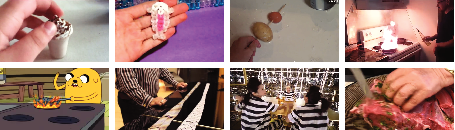
\includegraphics[width=0.5\textwidth]{figure_7_flt}
%  \end{subfigure}~
\caption{\textbf{Sample videos which our algorithm discards as an outlier for various queries.}
A toy milkshake, a milkshake charm, a funny video about How to NOT make smoothie, a video about the danger of a fire, a cartoon video, a neck-tie video erroneously labeled as bow-tie, a song, and a lamb cooking mislabeled as chicken.}
\label{outliers}
\vspace{-3mm}
\end{figure}

\vspace{-1mm}
\subsection{Qualitative Results}
\vspace{-1mm}
After independently running our algorithm on all categories, we discover activity steps and parse the videos according to discovered steps. We visualize some of these categories qualitatively in Figure~\ref{recipe:overall} with the temporal parsing of evaluation videos as well as the ground truth parsing.

To visualize the content of each activity step, we display key-frames from different videos. We also train a $3^{rd}$ order Markov language model~\cite{languageModel} using the subtitles and employ it to generate a caption for each activity step by sampling this model conditioned on the $\theta^l_k$. We explain the details of this process in \cite{supp}.

\begin{figure*}[ht]
  \begin{subfigure}[b]{\textwidth}
    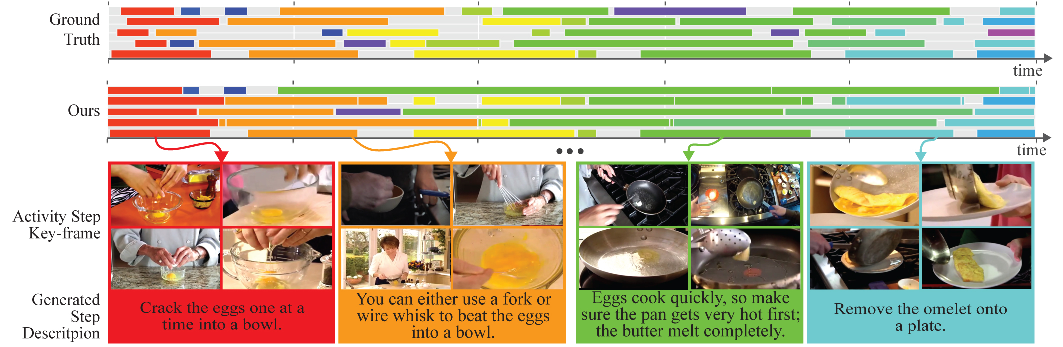
\includegraphics[width=\textwidth]{figure_8a_flattened}
    \vspace{-5mm}
    \caption{How to make an omelet?}
    \vspace{-1mm}
    \label{recipe:ommelette}
  \end{subfigure}

  \begin{subfigure}[b]{\textwidth}
    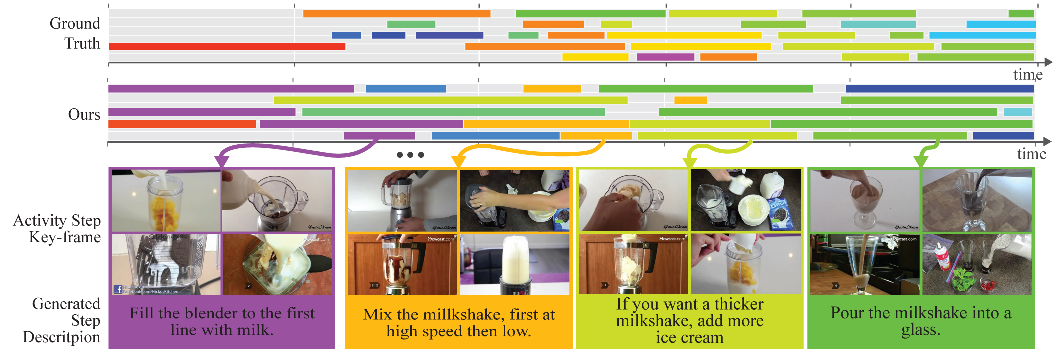
\includegraphics[width=\textwidth]{figure_8b_flattened}
    \caption{How to make a milkshake?}
    \vspace{-3mm}
    \label{recipe:milkshake}
  \end{subfigure}~
\caption{Temporal segmentation of the videos and ground truth segmentation. We also color code the activity steps we discovered and visualize their key-frames and the automatically generated captions. \emph{Best viewed in color.}}
\label{recipe:overall}
\vspace{-3mm}
%\normalsize}
\end{figure*}

As shown in the Figures~\ref{recipe:ommelette} and~\ref{recipe:milkshake}, resulting steps are semantically meaningful; hence, we conclude that there is enough language context within the subtitles in order to detect activities. However, some of the activity steps occur together and our algorithm merges them into a single step as a result of promoting sparsity.

\subsection{Quantitative Results}
We compare our algorithm with the following baselines.

\noindent\textbf{Low-level features (LLF):}
In order to experiment the effect of learned atoms, we compare them low-level features. As features, we use the Fisher vector representation of Dense Trajectory like features (HOG, HOF, and MBH) \cite{kantorov2014}.

\noindent\textbf{Single modality:}
To experiment the effect of multi-modal approach, we compare with single modalities by only using the atoms of one modality.

\noindent\textbf{Hidden Markov Model (HMM):}
To experiment the effect of joint generative model, we compare our algorithm with an HMM (using the Baum-Welch \cite{rabiner} via cross-validation).


\noindent\textbf{Kernel Temporal Segmentation \cite{potapov2014category}:}
Kernel Temporal Segmentation (KTS) proposed by Potapov et al.~\cite{potapov2014category} can detect the temporal boundaries of the events/activities in the video from a time series data without any supervision. It enforces a local similarity of each resultant segment.

\begin{figure*}[t]
  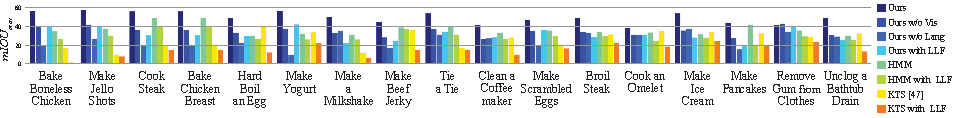
\includegraphics[width=\textwidth]{figure_9}
  \vspace{-9mm}
  \caption{$IOU_{cms}$ values for all categories, for all competing algorithms.}
  \label{mIOU}
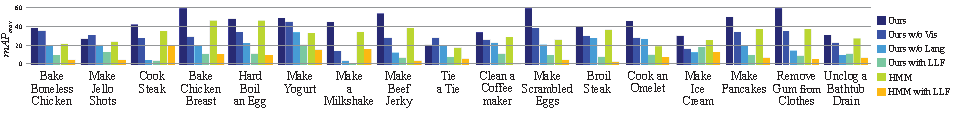
\includegraphics[width=\textwidth]{figure_10}
\vspace{-9mm}
\caption{$AP_{cms}$ values for all categories, for all competing algorithms.}
\vspace{-3mm}
\label{mmAP}
\end{figure*}

Given parsing results and the ground truth, we evaluate both the quality of temporal segmentation and the activity step discovery. We base our evaluation on two widely used metrics; intersection over union ($\mathbf{IOU}$) and mean average precision($mAP$). $\mathbf{IOU}$ measures the quality of temporal segmentation and it is defined as; $\frac{1}{N}\sum_{i=1}^N \frac{\tau^\star_i \cap \tau^\prime_{i}}{\tau^\star_i \cup \tau^\prime_{i}}$ where $N$ is the number of segments, $\tau^\star_i$ is ground truth  segment and $\tau^\prime_{i}$ is the detected segment. $\mathbf{mAP}$ is defined per activity step and can be computed based on a precision-recall curve \cite{THUMOS14}. In order to adopt these metrics into unsupervised setting, we use cluster similarity measure(csm)\cite{liao05} which enables us to use any metric in unsupervised setting. It chooses a matching of ground truth labels with predicted labels by searching over matchings and choosing the ones giving highest score. Therefore, $mAP_{csm}$ and $IOU_{csm}$ are our final metrics.

\begin{figure*}[t]
  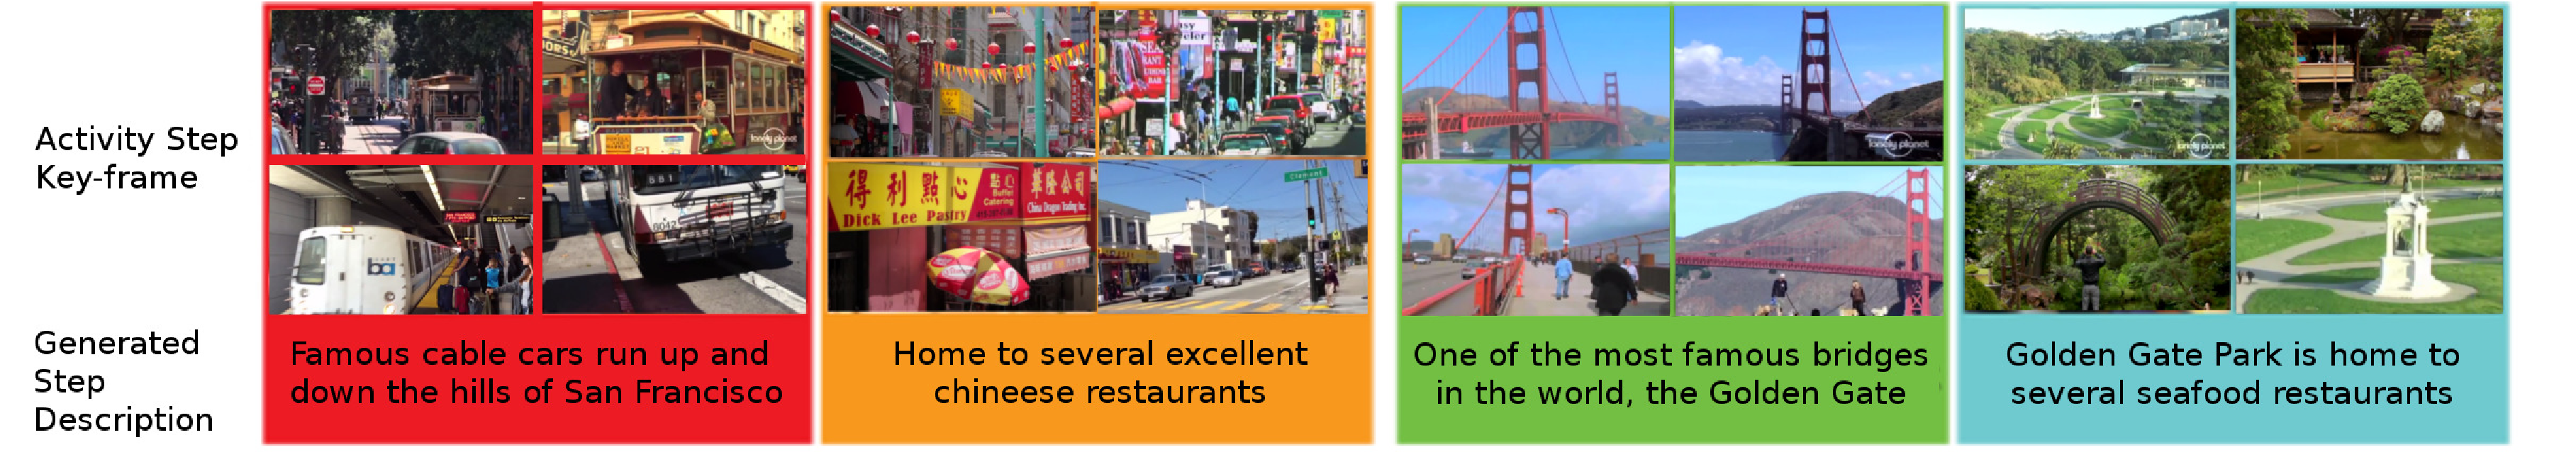
\includegraphics[width=\textwidth]{figure_8c}
  \vspace{-6mm}
  \caption{Qualitative results for parsing `Travel San Francisco' category.}
  \vspace{-2mm}
  \label{sf}
\end{figure*}


\vspace{1mm}
\noindent\textbf{Accuracy of the temporal parsing.}
We compute, and plot in Figure\ref{mIOU}, the $IOU_{cms}$ values for all competing algorithms and all categories. We also average over the categories and summarize the results in the Table \ref{averM}. As the Figure~\ref{mIOU} and Table~\ref{averM} suggest, proposed method consistently outperforms the competing algorithms and its variations. One interesting observation is the importance of both modalities reflected in the dramatic difference between the accuracy of our method and its single modal versions.

Moreover, the difference between our method and HMM is also significant. We believe this is due to the ill-posed definition of activities in HMM since the granularity of the activity steps is subjective. In contrast, our method starts with the well-defined definition of finding set of steps which generate the entire collection. Hence, our algorithm do not suffer from granularity problem.
\begin{table}
\caption{Average $IOU_{cms}$ and $mAP_{cms}$ over all categories.}
{\small
\resizebox{\columnwidth}{!}{%
\begin{tabular}{c|cc|cc|cccc}
 & KTS \cite{potapov2014category}    & KTS\cite{potapov2014category}     & HMM     & HMM    & Ours    & Ours     & Ours      & Our  \\
 &  w/ LLF &  w/ Sem &  w/ LLF &  w/Sem &  w/ LLF &  w/o Vis &  w/o Lang &  full \\
 \hline
$IOU_{cms}$  & 16.80 & 28.01      & 30.84 &   37.69   &  33.16 &  36.50 & 29.91& 52.36 \\
$mAP_{cms}$  &  n/a  & n/a        & 9.35  &   32.30   &  11.33 &  30.50 &  19.50 & 44.09 \\
\end{tabular}}}
\normalsize
\label{averM}
\vspace{-5mm}
\end{table}

\vspace{1mm}
\noindent\textbf{Coherency and accuracy of activity step discovery.}
Although $IOU_{cms}$ successfully measures the accuracy of the temporal segmentation, it can not measure the quality of discovered activities. In other words, we also need to evaluate the consistency of the activity steps detected over multiple videos. For this, we use unsupervised version of mean average precision $mAP_{cms}$. We plot the $mAP_{cms}$ values per category in Figure~\ref{mmAP} and their average over categories in Table~\ref{averM}. As the Figure~\ref{mmAP} and the Table~\ref{averM} suggests, our proposed method outperforms all competing algorithms. One interesting observation is the significant difference between semantic and low-level features. Hence, our mid-level features play a key role in linking videos.

\vspace{1mm}
\noindent\textbf{Semantics of activity steps.}
In order to evaluate the role of semantics, we performed a subjective analysis. We concatenated the activity step labels in the grount-truth into a label collection. Then, we ask non-expert users to choose a label for each discovered activity for each algorithm. In other words, we replaced the maximization step with subjective labels. We designed our experiments in a way that each clip received annotations from 5 different users. We randomized the ordering of videos and algorithms during the subjective evaluation. Using the labels provided by subjects, we compute the mean average precision $(mAP_{sem})$.

\begin{table}
\caption{Semantic mean-average-precision $mAP_{sem}$.}
\vspace{-3mm}
{\small
\resizebox{\columnwidth}{!}{%
\begin{tabular}{c|cc|cccc}
            & HMM     & HMM    & Ours    & Ours     & Ours      & Our  \\
            & w/ LLF  &  w/Sem &  w/ LLF &  w/o Vis &  w/o Lang &  full \\ \hline
$mAP_{sem}$ & 6.44   & 24.83  &     7.28 &   28.93  &  14.83    &  39.01 \\
\end{tabular}}}
\normalsize
\vspace{-5mm}
\end{table}

Both $mAP_{cms}$ and $mAP_{sem}$ metrics suggest that our method consistently outperforms the competing ones. There is only one recipe in which our method is outperformed by our baseline of no visual information. This is mostly because of the specific nature of the recipe \emph{How to tie a tie?}. In such videos the notion of object is not useful since all videos use a single object -tie-.
%over the entire video.
%This single object is a \emph{tie} and does not fit the assumption of a frame based on multiple visual atoms.

\vspace{1mm}
\noindent\textbf{The importance of each modality.}
As shown in Figure~\ref{mIOU} and \ref{mmAP}, the performance, consistently across all categories, drops when any of the modalities is ignored. Hence, the joint usage is necessary. One interesting observation is the fact that using only language information performed slightly better than using only visual information. We believe this is due to the less intra-class variance in the language modality (\ie, people use same words for same activities). However, it lacks many details(less complete) and is more noisy than visual information. Hence these results validate the complementary nature of language and vision.

\vspace{1mm}
\noindent\textbf{Generalization to generic structured videos}
We experiment the applicability of our method beyond How-To videos by evaluating it on non-How-To categories. In Figure \ref{sf}, we visualize the results for the videos retrieved using the query ``Travel San Francisco". The resulting clusters follow semantically meaningful activities and landmarks and show the applicability of our method beyond How-To queries. It is interesting to note that Chinatown and Clement St ended up in the same cluster; considering the fact that Clement St is known for its Chinese food, this shows successful utilization of semantic connections.
\vspace{-2mm}
